\documentclass[11pt, oneside]{article}
\usepackage[margin=1in]{geometry}
\geometry{letterpaper}
\usepackage{graphicx}
\usepackage{amssymb}
\usepackage[parfill]{parskip}
\usepackage{amssymb}
\usepackage{amsmath}
\usepackage{listings}
\usepackage{color}
\usepackage{standalone}
\usepackage{gensymb}
\usepackage{tikz}
\usetikzlibrary{matrix,chains,positioning,decorations.pathreplacing,arrows}
\usepackage{wrapfig}
\usepackage{epstopdf}

\graphicspath{ {images/} }

\def\layersep{2.5cm}

\sloppy
\definecolor{lightgray}{gray}{0.5}
\setlength{\parindent}{0pt}
\definecolor{dkgreen}{rgb}{0,0.6,0}
\definecolor{gray}{rgb}{0.5,0.5,0.5}
\definecolor{mauve}{rgb}{0.58,0,0.82}

\lstset{frame=tb,
  language=Matlab,
  aboveskip=3mm,
  belowskip=3mm,
  showstringspaces=false,
  columns=flexible,
  basicstyle={\small\ttfamily},
  numbers=none,
  numberstyle=\tiny\color{gray},
  keywordstyle=\color{blue},
  commentstyle=\color{dkgreen},
  stringstyle=\color{mauve},
  breaklines=true,
  breakatwhitespace=true,
  tabsize=3
}

\title{Neuro 120 Homework 3: Vision and Deep Networks}
\author{William Schmitt and Will Drew}
\date{Due: Thursday 8 November 2018}

\begin{document}
\maketitle

\section{Question 1: Early Vision and Convolutions}

\subsection{Difference of Gaussians Filter}

We created the difference of Gaussians filter via the following line of code: \lstinline{dog = fspecial('gaussian', [51 51], 3) - fspecial('gaussian', [51 51], 7);} and plotted this with \lstinline{surf(dog)} to produce the following image in Figure \ref{fig:dog}.

\begin{figure}[ht!]
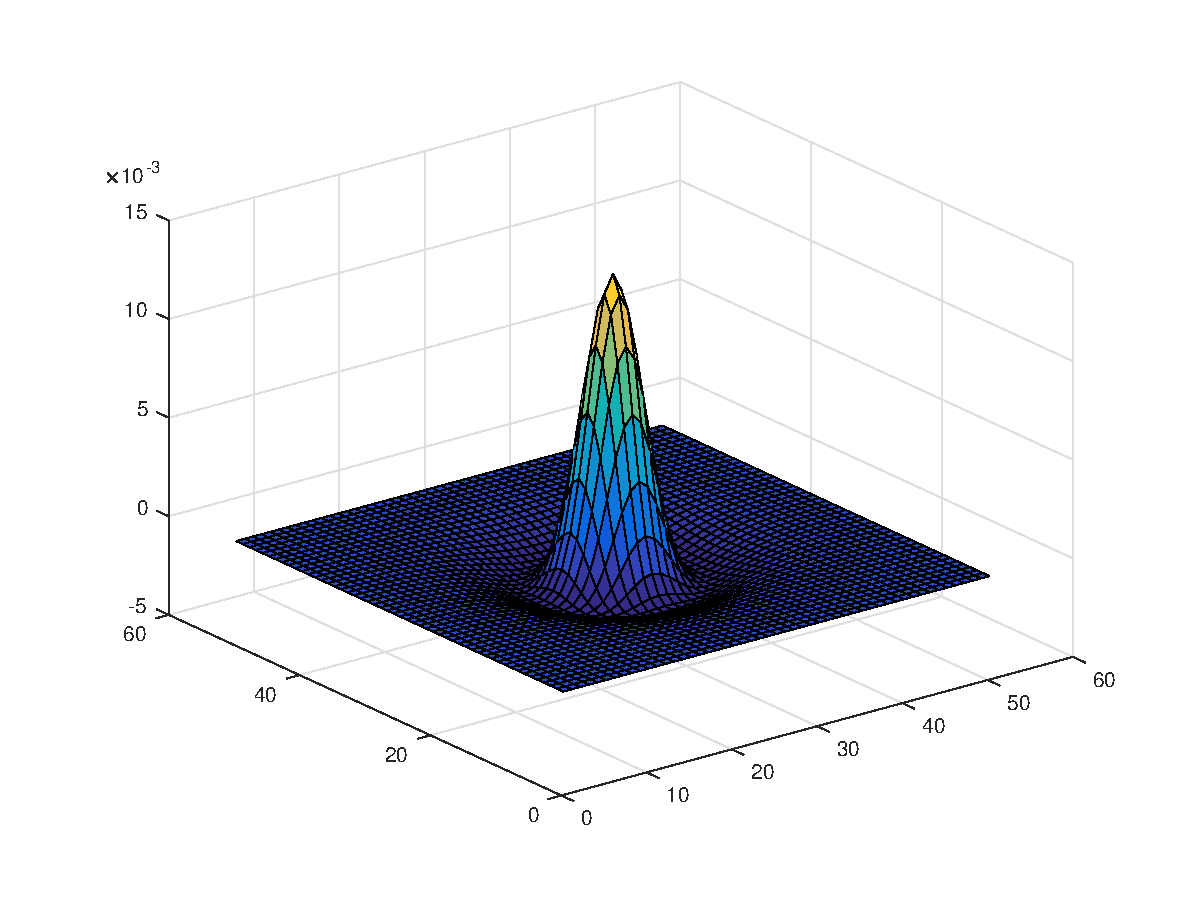
\includegraphics[width=1\textwidth]{dog.eps}
\caption{The coefficients of the difference of Gaussians filter.}
\label{fig:dog}
\end{figure}

\subsection{Mach band Convolution}

We convolve the Mach band image with the filter from part A via the following line of code: \lstinline{res = conv2(im_mach, dog, 'valid');}. We then plot this with the command, \lstinline{imagesc(res)}. This produces Figure \ref{fig:machConv}. We can see from this figure that the Mach band illusion results in activity at the boundary of the lines in the images (as seen by the one white line, corresponding to an increase in the RGC responses, and by the one black line, corresponding to a decrease in the RGC responses). Thus, these RGCs are detecting two ``edges'' in the Mach band illusion. This illusion is due to the center-surround nature of the difference of Gaussians filter the RGCs are modeled with.

\begin{figure}[ht!]
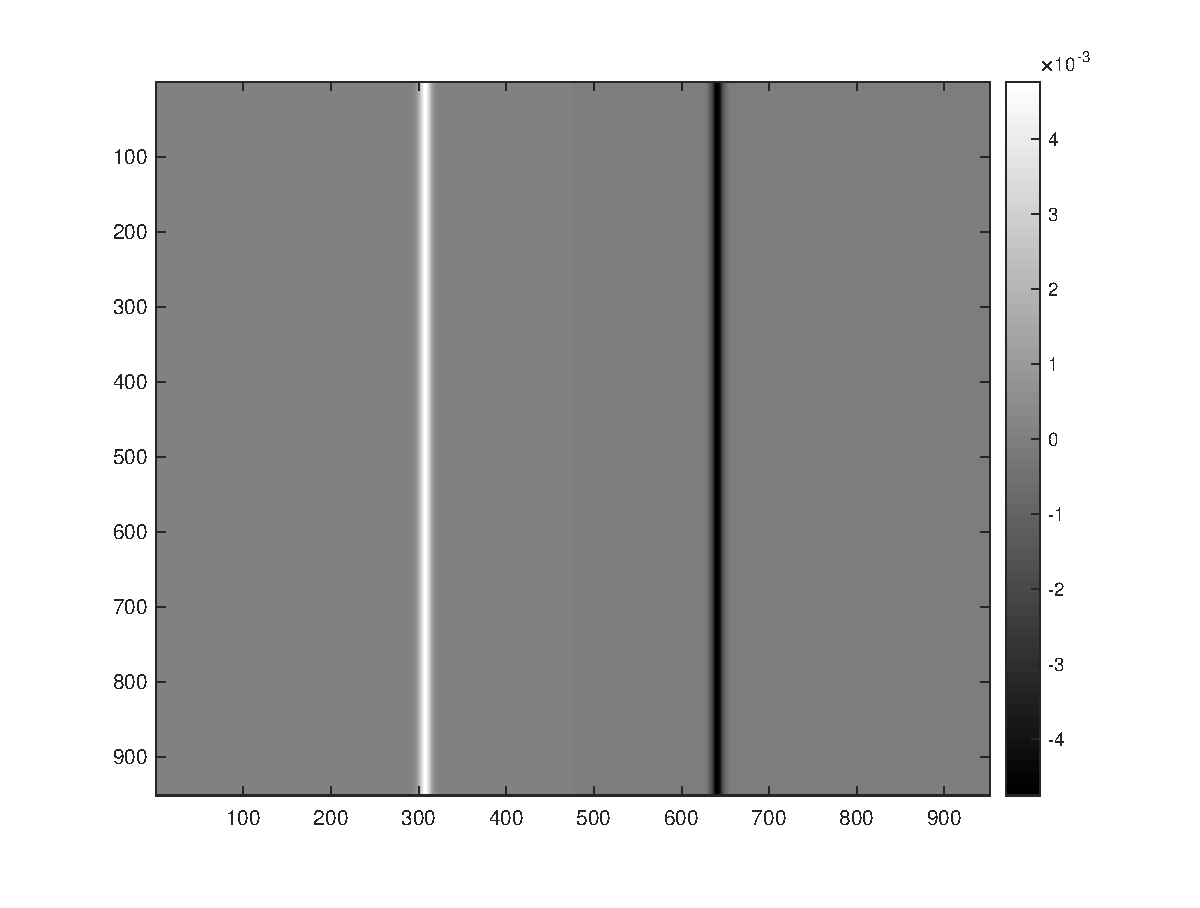
\includegraphics[width=1\textwidth]{mach_dog_conv.eps}
\caption{The result of convolving the Mach bands image with the filter from part A.}
\label{fig:machConv}
\end{figure}

\subsection{Mach band Convolution with a Small Constant}

We convolve the Mach band image with the filter from part A plus a small constant of $0.00001$ via the following line of code: \lstinline{dog2 = dog + 0.00001; res = conv2(im_mach, dog2, 'valid');}. We then plot this with the command, \lstinline{imagesc(res)}. This produces Figure \ref{fig:machConv2}. We can see from this command that again, the RGC model is detecting the two edges in the same locations. However, there is now a background gradient from light to dark (going left to right), with the increase (decrease) in activity being noticeably more at the first (second) edge. This relates to the Mach band illusion in that it is this detection of an edge in an image which has a larger overall gradient of brightness, which causes the person to perceive one side of the edge to be brighter than it actually is and one side to be darker than it actually is. 

\begin{figure}[ht!]
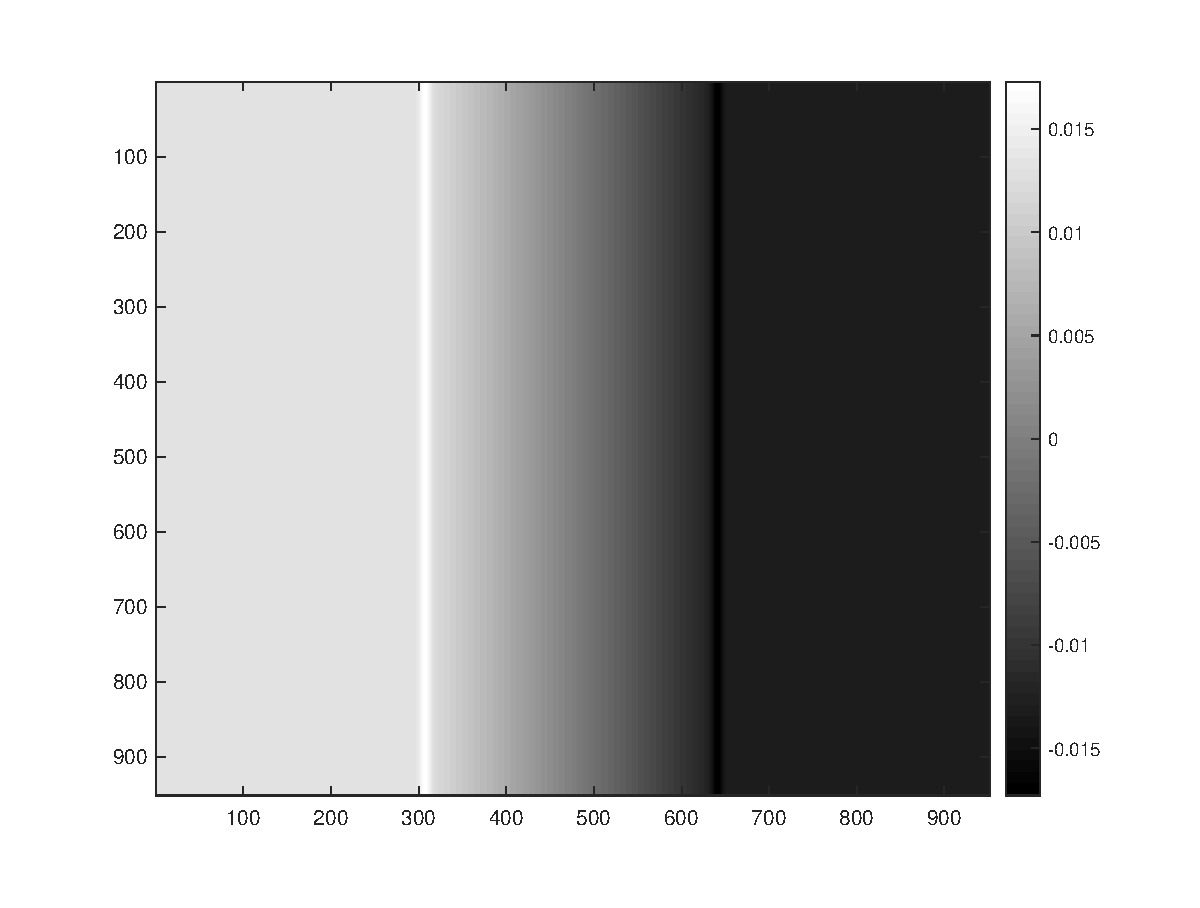
\includegraphics[width=1\textwidth]{mach_dog_conv2.eps}
\caption{The result of convolving the Mach bands image with the filter from part A plus a small constant.}
\label{fig:machConv2}
\end{figure}

\subsection{Checkerboard Illusion}

We convolve the checkerboard illusion with the filter from part A via the following of code: \lstinline{res = conv2(im_cb, dog, 'valid');}. We then plot this with the command, \lstinline{imagesc(res)}. This produces Figure \ref{fig:checkConv}. We can see from this figure that there are slight (barely noticeable) gray circles at the intersection of the lines compared to the middle of a stripe. Thus, we see that the center-surround nature of the RGCs produce a decreased response at the intersection of these stripes, which is why it appears to our eyes that there are gray circles at the intersections when they are really just white.

\begin{figure}[ht!]
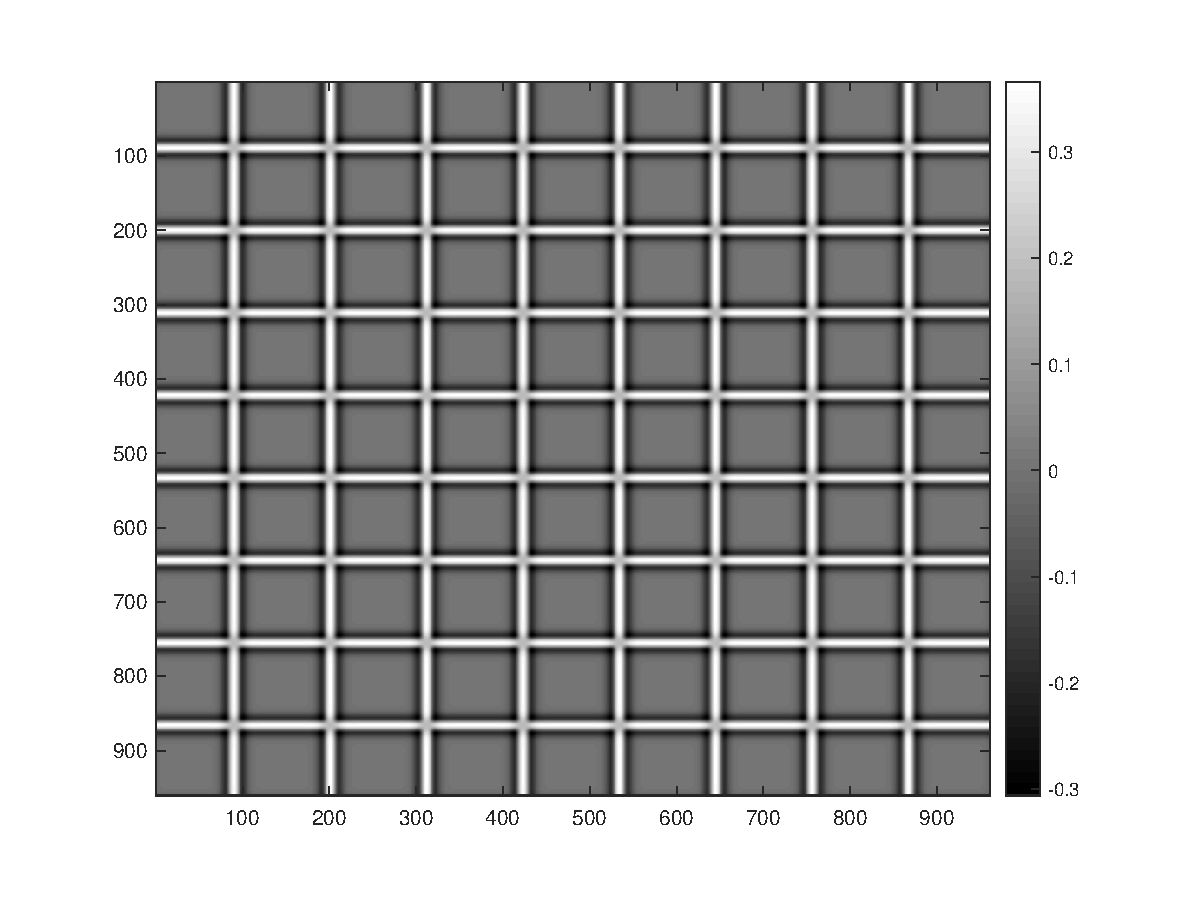
\includegraphics[width=1\textwidth]{check_dog_conv.eps}
\caption{The result of convolving the checkerboard illusion image with the filter from part A.}
\label{fig:checkConv}
\end{figure}

\subsection{Checkerboard Illusion with a Broader Filter}

We make a new difference of Gaussians filter with the following code: \lstinline{dog3 = fspecial('gaussian', [51 51], 3) - fspecial('gaussian', [51 51], 7);}. We plotted this with \lstinline{surf(dog3)} to produce the following image in Figure \ref{fig:dog3}. We then convolve the checkerboard illusion with this filter via the following code: \lstinline{res = conv2(im_cb, dog3, 'valid');}. This produces Figure \ref{fig:checkConv2}. We can see from this figure that 

\begin{figure}[ht!]
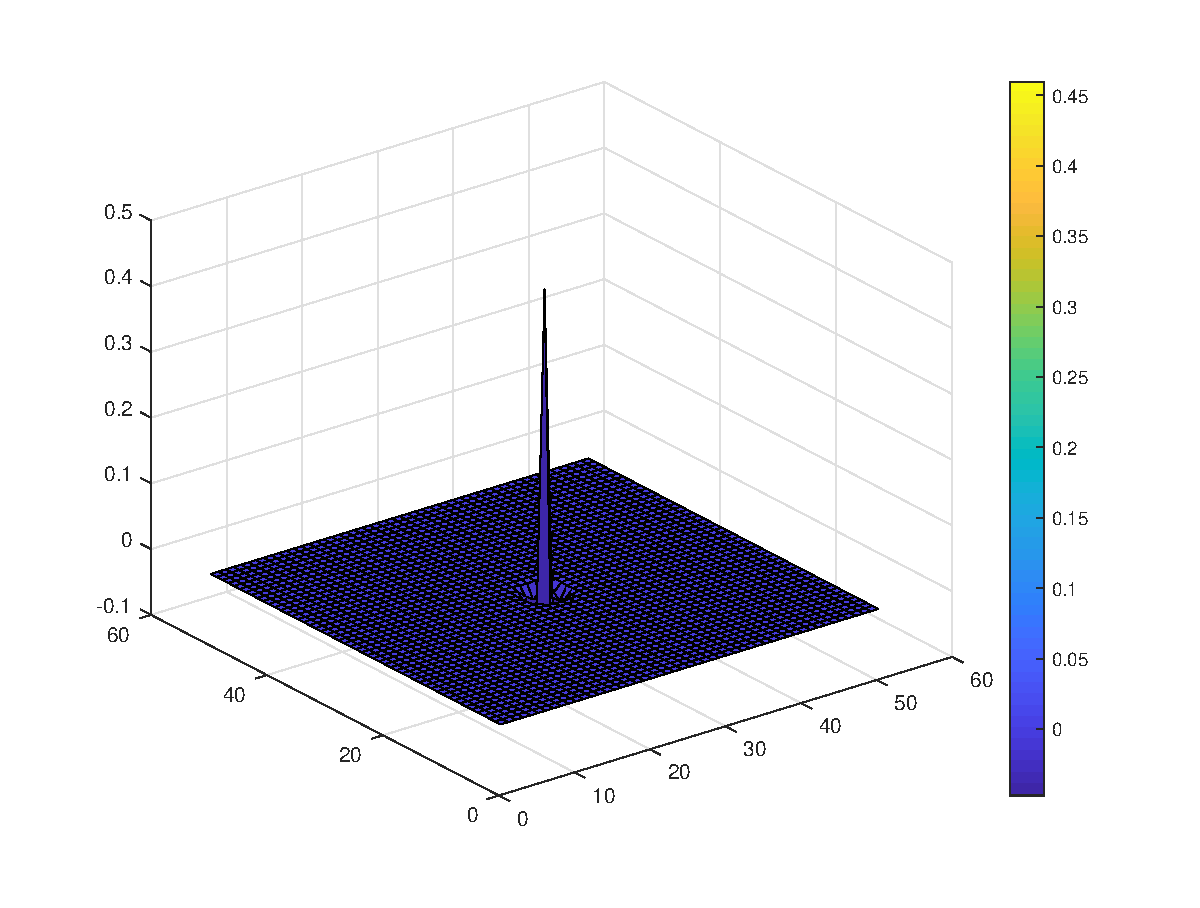
\includegraphics[width=1\textwidth]{dog3.eps}
\caption{The coefficients of a broader difference of Gaussians filter.}
\label{fig:dog3}
\end{figure}

\begin{figure}[ht!]
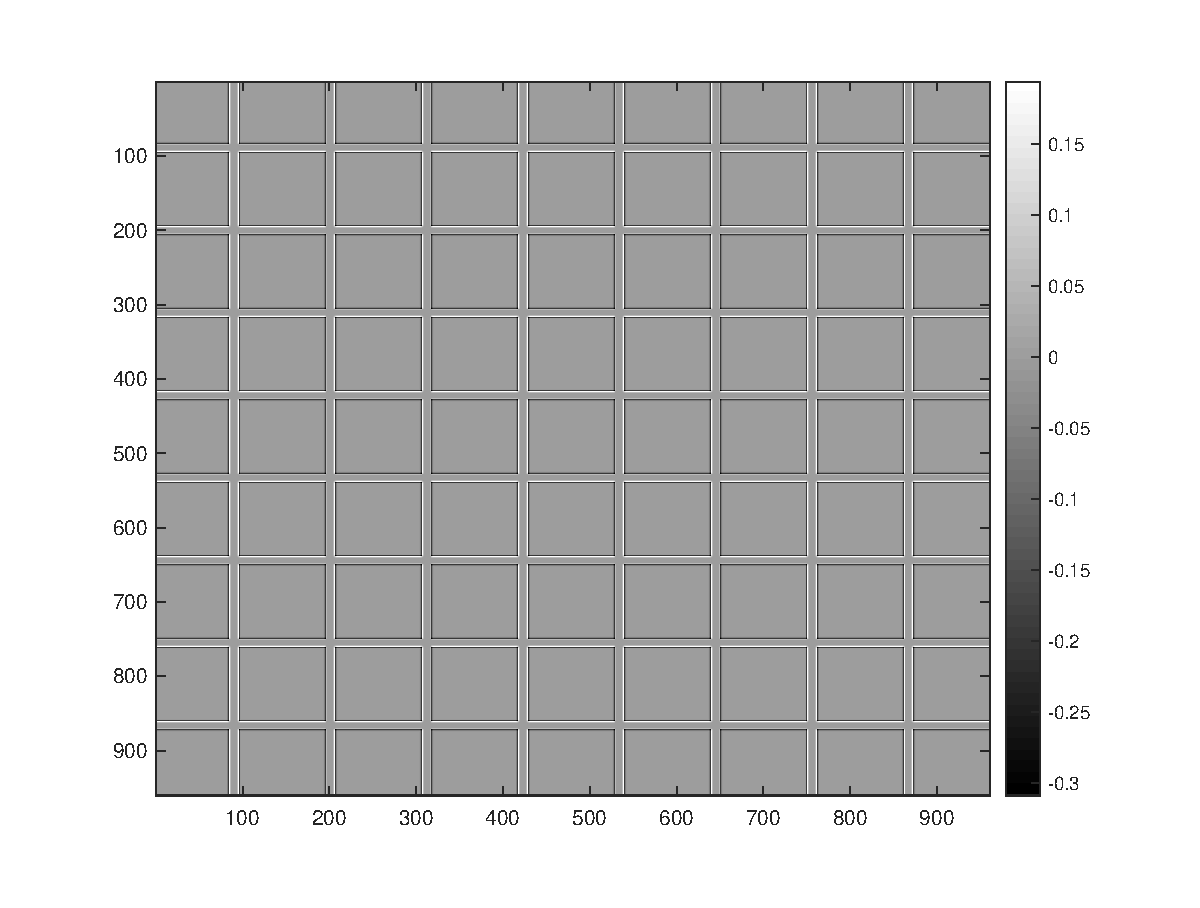
\includegraphics[width=1\textwidth]{check_dog3_conv.eps}
\caption{The result of convolving the checkerboard illusion image with a broader filter.}
\label{fig:checkConv2}
\end{figure}

\end{document}
